\providecommand*{\listingautorefname}{Code sample}

\newcommand{\trait}[1]{{#1}}

\newcommand{\type}[1]{{#1}}
\newcommand{\fun}[1]{{#1}}
\newcommand{\kubecomp}[1]{{#1}}
\newcommand{\actor}[1]{{#1}}
\newcommand{\msg}[1]{{#1}}

\chapter*{Abstract}
\label{abstract}


\chapter{Introduction}
\label{chapter:introduction}
Financial markets are complex systems, in which, market players interact with each other to determine
price of an asset. Advances in financial technologies, like the advent of blockchain technology,
and corresponding proliferation of cryptoccurencies , like Bitcoin\cite{bitcoin} have changed nature of trading.

As a result of these advances, financial markets are now more approachable than ever, and thus present a significant
opportunity. One example of services that successfully exploit this opportunity are cryptocurrency exchanges. They
are a whole new kind of marketplace, that provides several advantages to its users. These exchanges usually provide
approachable Web based user interface for everyone and, HTTP/WebSocket API for advanced users.

In order to capitalize on these advances, we must use advanced trading techniques. One of these is algorithmic
trading. Basis of algorithmic trading, is utilization of some kind of algorithm, along with market data, in
order to determine most profitable actions, that should be performed on the market.

This approach, has several requirements. One of them is large amount of computing power, since used algorithms
might be extremely complex. Latency is also a big concern, since this space is extremely competitive, and a party,
which is able to perform optimal actions sooner than all other parties, will net a larger profit.
Thanks to these requirements, usage of this technique is not easy, or cheap.

However, advances in development and usage of distributed systems, might be an easy solution to these problems.
Cloud computing\cite{wiki:cloud} is now more widespread, and easy to use than ever. Thanks to new technologies like
docker\footnote{https://www.docker.com/} and kubernetes\cite{web:k8s}, the creation and management of distributed systems is easy,
and systems created with these technologies can be easily secured, are scalable and provide other benefits
for developers creating them compared to more monolithic architectures.

\section{Objectives}
This thesis is concerned with creation of a system for algorithmic trading. This system was concieved
as a distributed application. Usage of distributed was chosen in order to minimize cost of
approach should help with performance requirements,
and the difficulty of implementing such complex system. The system should be designed with latest technological advances in mind, and
should utilize cloud computing environment.

The system itself should be extensible and scalable. The extendability requirement deals with ability to integrate new markets,
with types of assets, or add new functionality to existing ones. The scalability of the system deals primarily with the system's
ability to automatically scale based on amount of users and resulting load on the system.

From users' perspective, the system should be a easy to use web application. The user should be able to define custom
algorithms and strategies, and apply them to different markets.

\chapter{Current state \& existing solutions}
\label{chapter:current_state}
Existing solutions for algorithmic trading that are aimed to regular users instead of specialized investment companies
have been available for some time. These solutions range from simple command-line applications that connect to single exchange
to large distributed deployments with web interface that connect to largest stock exchanges\cite{Agopyan_financialbusiness}.

\section{Examples}
We chose to look at a few solutions from different part of this spectrum in order to better understand the requirements
that will be placed upon the designed system. All evaluated solutions perform algorithmic trading of cryptocurrencies.
While restricting our research to this small part of global markets might affect our findings, the primary
market in which the designed system will operate also is a cryuptocurrency market.

\subsection{Gekko}
On the lower end of the spectrum, there is a simple application written in javascript called Gekko\footnote{https://gekko.wizb.it/}.
This application is open source and runs on top of the Node.js. The application can import historical data,
and use this historical data to backtest\todo{Footnote} created strategies. The strategies are written in Javascript, with the support
of a simple library that contains implementations of financial indicators, that are commonly used with these types
of trading strategies.

It also provides simple web interface, but can only connect to one exchange at a time, and only supports one user at a time.

Therefore, it lacks the scalability of a distributed approach.

\subsection{CryptoTrader}
On the higher end of the scale spectrum, we have CryptoTrader\footnote{https://cryptotrader.org/}. This solution
is implemented as a web application, that supports multiple users at the same time. Each user can define multiple
strategies, and each strategy can utilize multiple data sources. The strategies are written in language called
CoffeeScript, with slightly inconvenient but very powerful API. This system serves as a good benchmark for
our system.


\chapter{Theory}
\label{chapter:theory}
This chapter describes theoretical approach to different parts of target system.
\section{Trading \& Exchanges}
In order to define algorithmic trading, we must first define what trading is, and how it is performed.
Trading is performed on exchanges. Key aspect of exchange trading is the price discovery mechanism. For all assets,
traded on an exchange, the price is not dictated by any single party. Instead, the price is "discovered" by interaction of
buyers and sellers. Buyers advertise the highest price they are willing to pay for an asset, and sellers advertise the lowest price
they are willing to accept. These 2 prices correspond to basic economic principle of supply and demand. When there are more sellers active
on the exchange, the price will fall, since there are isn't enough buyers to buy an asset. This principle also applies in reverse, if there are more
buyers active on the market, the price will rise.
The maximum price listed by a buyers known as \textbf{bid} price, and the minimal price listed by a seller is known as \textbf{ask} price

Since these exchanges are dynamic environments, with always fluctuating pressures on either side, the price of an asset, varies over a time.
The amount of this variance is called \textbf{volatility}.

Historically, the exchanges were physical, mainly used for trading stocks, and
were called stock exchanges. They were physical locations , where individual traders met, and traded one asset for another.
Primarily, these trades consisted of stocks or goods against money. Another type of trade is when 2 parties trade one currency for another.
Exchanges specializing in these types of trades are called \textbf{FOREX} (Foreign exchange) markets.

Most recent of exchange types, is the cryptocurrency exchange. These exchanges are almost always purely virtual. All trading is performed
via web interface. The main advantage for our purposes is the ease of use of these exchanges, and their modern features.
Virtually all of them provide multiple APIs for different purposes. A real-time API for low-latency streaming of updates to clients,
and a REST API provided for executing trades on the exchange.

\subsection{Algorithmic trading}
First financial markets with electronic execution and connection to communication networks appeared
in late 1980s and 1990s. This allowed some degree of automation, but weren't yet used for fully
automated trading. In 2001 a paper published by IBM\cite{Tesauro:2001:HBA:501158.501183},
encouraged adoption of algorithmic trading. In this paper, fully automated trading strategies
consistently outperformed human counterparts. Since then, the amount of trading performed by
automated systems has steadily risen.

As algorithmic trading became more common, new trading strategies started popping up, and
an arms race was started. In this arms race, the parties were consistently introducing new,
more effective ways of performing trading decisions, and executing resulting trades. The \textbf{HFT}(High frequency trading)
is a culmination of the automated trading arms race.

\subsubsection{High frequency trading}
This form of trading is characterized by high turnover and order-to-trade ratios(number of created orders compared to executed trades).
It utilizes highly specialized order types, co-location of trading equipment as close as possible to exchange.
In 2010, only 2\% of US based trading firms specialized in HFT, but these 2\% accounted for more than 73\% of all
trading volume\cite{article:computerized_trading}.

There are four key categories of HFT strategies\cite{wiki:hft}:
\begin{itemize}
    \item {Order-flow based market making -
    Utilizes data about amount \& volume of newly created orders to determine state of the market \& then
    creates orders on a regular basis to capture bid-ask spread }
    \item {Tick data based market making - Utilizes tick data (current bid \& ask prices) to determine state of the market
    creates orders on a regular basis to capture bid-ask spread }
    \item {Event arbitrage - Utilizes external information, about events that might affect the market to
    create specialized orders to profit from this event (Company mergers)}
    \item {Statistical arbitrage - Utilizes multiple asset classes, to create complex transaction chains, which allow for relatively risk free profit }
\end{itemize}

Our system will mainly support strategies, that would fall into \textbf{Tick data market making} category. This is due
to simplicity of these strategies, and the fact that the information provided by the cryptocurrency exchanges is best suited
for these strategies.
\todo{Reword}
Strategies will be used to create trading decisions for multiple assets. The fact that
there are multiple different strategies evaluated for multiple currencies means that the total number of strategy evaluations is
extremely large. In addition to that , the system will also have to provide some degree of scalability, since the system will
have to respond to changes in number of users.

To satisfy these constraints, the system will have to be of distributed nature.

\section{Distributed systems}
Distributed systems are systems, that are comprised of many loosely coupled components. These components might be threads
in single process, processes on single computer, or multiple computers connected through shared memory or a network.
These components communicate by utilizing shared memory, or by passing messages to one another. Components interact with
one another in order to achieve shared goal. Distributed systems have several key properties\cite{Coulouris:2011:DSC:2029110}:

\begin{itemize}
    \item Concurrency - The computation in one component is concurrent with computations performed by other components
    \item No global clock - There is no single global clock, each component has only local clock
    \item Independent failures - Failure of one component does not imply failure of other components
\end{itemize}

We can use these properties to make a very loose definition of what a distributed system is. In order to better understand these
types of systems, we will have to analyze several additional properties.

\subsection{Additional properties}

We can analyze whether a distributed system uses homogeneous or heterogeneous components.
The systems that only use homogeneous component are commonly used in open
environments, like the Internet. Systems like BitTorrert or similar file distribution software are the perfect example.

In order to find an example of heterogeneous system , we don't have to look further than World Wide Web. In this system,
we have servers and clients, which are 2 different types of system components.

Another property of distributed system is the communication method. There are 2 primary approaches to communication between 2 components. Message passing or shared
memory. Most commonly used is message passing, since it allows for 2 components to be on different networked computers, while implementations that utilize
shared memory can only be used on a single machine. We can simulate former approach with the latter and vice versa at the cost of performance.
Going further, this thesis will only deal with systems that use message passing as the communication paradigm.

Another aspect of component communication is the communication protocol. This does not mean the underlying technology that is used to send
messages, but rather the protocol that determines what messages will be sent , and when.

Components might communicate using simple request - reply based protocol , like HTTP. Or they might communicate using slightly different
publish - subscribe model over technologies like ZeroMQ, or message buses like Kafka.

We can also examine the rigidity of the system. The number and types of components can be either dynamic, or static. This
property influences the \todo{Self healing architectures need dynamic components, figure out wording}

Using these properties, we settled on a model of a distributed system, that utilizes large amount of heterogeneous components.
Each of these components communicates primarily using request-reply style of communication utilizing message passing paradigm.
This paradigm is called the Actor model.

\section{Actor model}
Actor model is a conceptual model of describing concurrent computation. It treats Actors as primitives of concurrent
computation. Each actor can: Create new actors, send messages, modify its state and decide, how to respond to
received messages. Primary constraint is the restriction of modifying application state.
Each actor can modify its local state however it wants, but can only affect other actors by sending messages.

Thanks to this property of isolation, there are no necessary locks to ensure memory safety.
It originated in 1973, and has been used for understanding distributed computation, and also as
a basis of several implementations of concurrent systems.

According to Hewitt\cite{journal:actor}, the actor model is based on physics. This contrasts
other computational models, which are most commonly based on mathematical logic, set theory or similar concepts.
The primary takeaway from physics , that can be observed in actor model, is taken from quantum physics, and it
is the idea of uncertainty. We cannot observe precise state of a whole system, because attempting to do so
will affect it, and therefore invalidate measured results.

\subsection{Alternative models}
Actor model is very high level, and shares both goals and properties with other programming paradigms. These
include:
\subsubsection{OOP}
If we consider Smalltalk, and its message passing model of object oriented programming, we observe several common properties.
\begin{itemize}
    \item Encapsulation - Both actors and objects can only directly manipulate their local state
    \item Message passing - Both actors and objects can send messages to other actors and objects respectively
    \item Polymorphism - Both actors and objects can decide, how will they respond to specific message
\end{itemize}

While these models are similar, Smalltalk was tied to particular implementation, and it did not provide
tools for concurrent programming. But the similarity nonetheless still stands, and actor model can be also understood as
an extension of OOP paradigm.

\subsection{Petri nets}
Petri nets have been widely used to model concurrent computation. However, while they are extremely well suited
for modeling control flow, They can't be used to model data flow in their basic form. Another problem is
simultaneous action. While we can easily simulate simultaneous action of removing a marker from one place, performing
a transition and placing a marker in output place, in reality, these 3 actions will not be simultaneous.

\subsection{Communicating sequential processes}
While CSP model has similar goals to actor model, there are several ways, in which these 2 models differ.
Most important difference is that Actor model is inherently
dynamic, while CSP model if based on a fixed number of sequential processes communicating in a fixed topology\cite{Hoare:1985:CSP:3921}.
Usage of this model therefore is not particularly suited for our purposes, since designed system should be dynamically scalable,
which is not possible in CSP model.

\subsection{Implementations}
While the actor model is almost 4 decades old, implementations of concurrent and distributed systems that
are based on this model are more common than ever.
\todo{Reword}
Originally, this model was primarily used in niche systems, like
telecommunications

The success in these kinds of systems slowly fueled growth of this paradigm into more general purpose programming. With this
growth, several libraries started popping up. There are multiple similar libraries in
wide variety of languages, ranging from Lisp to C++. Today, one of the most commonly used libraries is Akka\cite{web:akka}, which was originally
developed for Java and Scala, but was reimplemented using C\# for the .NET platform. While Akka is extremely easy to use,
extensible, and performant, it is still only implemented for managed languages, which require heavy runtime with tracing garbage collection.

\todo{Erlang here}

This was one of the aspects , which influenced the decision to look for another library, that would be implemented in
non-managed language. The library, we chose is called Actix\cite{web:actix}, and is implemented in Rust\cite{Blandy:2015:RPL:3019371}
programming language.

\section{Rust}
Rust is a new programming language developed by Mozilla. It was created as a response to many shortcomings of existing low level
languages such as C and C++. While these languages have crucial place in programming landscape, providing the highest performance and
degree of control over hardware, they are outdated, unergonomic and unsafe ( particularly with respect to concurrency). On opposite
side of this equation , are managed languages, that are highly ergonomic, and seem to contain most innovation in this space.

Rust language aims to position itself among the low level languages, bringing new and exciting features to this space.
It was originally developed by Graydon Hoare\cite{web:rust_progress} while working at Mozilla, and was based on
ML. Probably the most important step, was adoption of the language by Mozilla for the purpose of creating new browser engine
called Servo\cite{proc:servo}. Goal of Servo was to experiment and innovate in the Web browser space, without
the depending on over 30 years of legacy code, that was Firefox.

\subsection{Language basics}
Basic concepts of the Rust language are very similar to other C based languages. Basic structure is denoted by braces,
It has functions, a module system, and other features, that will be uninteresting to intermediate programmer.
However, some of the more advanced concepts make this language particularly well suited for large concurrent systems, and
will be explored later in this chapter.

Language has 2 primary conceptual entities -- types, and traits.
For the types, language supports product and sum types(structs and enums respectively), and references (which can be mutable or immutable).
Traits are more interesting feature. They are similar to interfaces in Java, but their closest analogy would be typeclasses from Haskell.
Traits are used to declare a set of constraints, types, constants, and functions, that an implementing type(implementor) must provide.
Each implementor, can implement any number of traits.

The language supports all the most common control flow constructs like conditionals and loops. In addition to that, it
also supports expressive pattern matching using the \verb|match| expression. However, it does not support the
\verb|goto| control flow construct for unrestricted jumps.

\subsection{Features}
The requirements influenced the design of the language in a significant way. It started out as general purpose programming
language with functional features, very similar to ML, and then acquired some features that make it excellent
systems programming language. These features are:

\begin{itemize}
    \item Generic programming based on traits
    \item Memory model that allows safety without garbage collector
    \item Primitives to eliminate data races
    \item Integrated build system and package manager
\end{itemize}

\subsection{Generic programming, traits}
Generic programming is a paradigm, in which algorithms are written in terms of unspecified types.
The types are then specified upon instantiation. These types are called type parameters, or generic types.
By using this tool, programmer can write common functions or types only once, and use them with multiple
types, thus reducing duplication. This paradigm was pioneered by ML, and is supported in virtually every
modern language in one shape or form.

Modern implementations follow 2 primary approaches for typing generic constructs: Structural, or protocol based.

Structural generic typing (also called Duck typing) is primarily used in C++. With this approach, the type
checking is performed after instantiation of generic construct. This allows for greater flexibility.
But virtually all implementations of this approach suffer poor diagnostic messages\cite{Traver:2010:CEM:1863617.1945532}.

Protocol(Interface) generic typing is an approach , in which the generic construct itself undergoes type checking, and
every instantiation requires minimal amount of additional checks. This requires programmer to describe the required interface
of each type parameter explicitly. These requirements take form of Interfaces (Java, C\#), Concepts (Future C++),
Type classes (Haskell) or Traits(Rust). Then, upon instantiation it is only necessary to check whether
each type parameter satisfies specified constraints.

\subsection{Traits}
As described earlier, traits are used to declare interface, that a type must provide. They are used tu support
other language features, and must be understood in order to effectively use the language.
Below is an example of a simple trait.


%@formatter:off
\begin{code}[language=rust,label={ord_trait},caption={Trait definition}]
    pub trait Ord: Eq + PartialOrd<Self> {
        fn cmp(&self, other: &Self) -> Ordering;
        fn max(self, other: Self) -> Self where Self: Sized {
            if other >= self { other } else { self }
        }
    }
\end{code}
%@formatter:on

\autoref{ord_trait} Shows definition of an Ord trait that defines complete ordering over implementors type. This trait specifies Additional constraints for implementing types
(Also called supertrait constraints). Every type that implements Ord, must also implement Eq, and PartialOrd trait with generic
argument of impelementing type. The implementor, must provide implementation for \fun{cmp} method, that takes an one argument of implementors type,
and returns an ordering. The trait definition also specifies \fun{max} method for types, that implement Sized trait, and provides default
implementation.
The Self keyword is used to refer to implementing type in the trait definition.
Traits can also be generic, accepting type parameters, such as the PartialOrd trait used earlier.

%@formatter:off
\begin{code}[language=rust,label={ord_impl},caption={Trait implementation}]
    impl Ord for bool {
        fn cmp(&self, other : &bool) -> Ordering {
            if self & !other {
                return Ordering::Greater;
            }
            if self == other {
                return Ordering::Equal;
            }
            return Ordering::Less;
        }
    }
\end{code}
%@formatter:on

\autoref{ord_impl} shows simple implementation of Ord trait specified earlier for boolean data type. This sample
uses an impl block, to implement a trait for specific type. Impl block can be generic, and have to provide
implementations for all functions that do not have default implementations specified in trait definitions.

\subsection{Marker traits}
The traits \trait{Eq} and \trait{PartialOrd} used earlier are self-explanatory, they denote the availability of equality comparison, and partial order
in implementing types. However, the \trait{Sized} trait might not be so easy to comprehend.

This trait belongs to special category of traits, called marker traits. These include \trait{Send} , \trait{Sync}, \trait{Sized} and several others.
The marker traits do not provide any functions and serve, as their name implies, as markers. They are used for marking specific
types. The \trait{Sized} trait marks types, which have their sizes defined at compile time, and is automatically implemented
for these types by compiler. The example of unsized type might be \type{[u8]} , which is an arrray with unknown length.

The \trait{Send} and \trait{Sync} traits are crucial for features supporting safe concurrent programming , and will be explored later in
this chapter.

\subsection{Memory management}
Modern programming languages primarily use one of 2 approaches to manage memory.

The garbage collection is an approach most commonly used in High-level languages. 2 Most common implementations
are reference counting and tracing garbage collection. Both of these approaches have drawbacks, primary ones being
difficulty handling reference cycles for reference counting and necessary program pauses for tracing garbage collection

Second common approach used is called RAII, which stands for "Resource acquisition is initialization". It is most
prominently associated with C++, but is used in D, Ada, and Rust. This approach was originally developed for exception safe
resource management in C++\cite{stroustrup2015brief}.

RAII is more oriented for management of resources, but if we consider dynamically allocated objects a resource, it serves
the same purpose as garbage collection.

The lifetime of a resource is tied to object lifetime. The resource is acquired during creation of the object,
and released during destruction. The object can have unconstrained lifetime (Allocated on a heap), or scope constrained
lifetime (Allocated on the stack).

In C++ the creation and destruction of object is performed by specific functions(Constructor and destructor). Rust does
not support object oriented programming in a classical sense. The data types are created structurally(enumerating all component values).

The destruction of values is performed with the help of a trait system. If a type, implements the \trait{Drop} trait,
it must implement the \fun{drop} method, which has similar semantics to C++ destructor. This method will be invoked
when variable of this type goes out of scope, and memory associated with it will then be deallocated

\subsubsection{Move semantics}
Another important concept taken from C++ is move semantics. Until C++11, the only approach was copy semantics, in which
assignment to a variable from another variable would create copy of referenced object.
The drawback of this approach, is inability to express a type, that should not be copyable, but should be movable.

The move semantics on the other hand, can express this concept easily. With copy, the assignment to a variable, invalidates the
old variable. In C++ move semantics, the object referenced by old variable is replaced by and "Empty" object ( an object
that is safe to destruct, and its destruction will not invalidate copied object).

In rust, the invalidation of moved-from variables is enforced at compile time, and usage of invalidated variable will result in a
compiler error. Rust provides only move semantics, with copy semantics emulated by the \trait{Clone} trait.

\subsubsection{Ownership and borrowing}
Conceptually, the move semantic are used to express the concept of ownership. If a variable, contains an object, it "owns"
that object , and is responsible for its destruction. However, requiring programmer to transfer ownership of an object every time
it is passed into a function would be extremely tedious on programmer side, and copying of an object would degrade performance.

Rust also provides a way to reference objects, without moving or copying them. By using \verb|&| or
\verb|&mut| sigil, the programmer can create immutable and mutable reference respectively. Why 2 reference types? This is
done to ensure memory safety by disallowing mutation and aliasing at the same time.

We can create any number of immutable references to an object, but these references can't mutate referenced object, or
we can create one mutable reference, and use this reference to mutate the object. Creation of multiple mutable references
is not allowed, and will result in compiler error.

\subsection{Concurrency primitives}
The concept of ownership and borrowing is also used to ensure memory safety in multithreaded programs, and prevent
data races

Data race occurs when 2 or more threads concurrently access same location of memory, one of these accesses is a write,
and accesses are unsychronized. These types of bugs are extremely hard to discover, and have lead to death of several medical patients in
one extreme case\cite{article:therac}.

The ownership and borrowing system prevents these kinds of data races, but Rust also provides tools for ensuring other
constraints in multithreaded programs. Primary building blocks are 2 marker traits. The \trait{Send} and \trait{Sync} traits.

The \trait{Send} trait denotes that the implementor can be safely transferred to a different thread. This trait is automatically
implemented by compiler, when appropriate. For example, objects that reference thread local storage do not implement \trait{Send}.

The \trait{Sync} trait is implemented for types that can be safely shared between threads(Reference can be shared between threads).

These 2 traits are then used by library abstractions like \type{Mutex} and \type{Rwlock} to ensure memory safety and data race free code.
For example, the \type{Mutex} abstraction is used to protect an object with a mutex. The \type{Mutex} struct is generic,
with one type parameter, that denotes contained value, which must implement \trait{Send} trait.
This ensures that the contained value can be safely shared between threads. The mutex itself implements both \trait{Send} and \trait{Sync} traits,
meaning mutex can be safely shared between threads.

\subsection{Build system and package manager}
One area that low level languages are extremely outdated compared more high-level languages is modularity and code reuse.
While these languages provide tools for creating modules, that can be combined to form a larger program, they lack tools
for supporting this process. Because of this, the number of libraries, that a project uses is extremely low, and
each project ends up reimplementing existing functionality. This is a large problem in C++, where most common
libraries used are extremely large (QT, Boost), and domain specific libraries are virtually nonexistent.

Rust aims to solve this problem with \textbf{Cargo}. Cargo is primarily a build too and package manager, but it also
provides testing and benchmarking support. Cargo operates on Crates. A crate is the smallest compilation unit.
Each crate contains multiple source code files, and a manifest file which specifies metadata information about this crate, and lists dependencies.

Crates can be published and uploaded to \textbf{crates.io} repository, which is closely integrated with Cargo. Each crate can then
also require dependencies from this repository.

This improvement encourages development and usage of small, domain specific libraries, which in
turn allows for the standard library to be extremely small, on par with C++, without reducing productivity.

\section{Actix}
One of primary reasons for choosing rust was the choice of Actix\cite{web:actix} library. Actix is a library that provides abstractions
for implementing applications with Architecture based on actor model. It provides runtime system for managing actor, that is
based on Tokio libarry, which is core for asynchronous programming in rust(Similar to LibUV). It also provides
traits for defining actors, implementing their behavior in response to messages.

\subsection{Actor in actix}
Actor in actix is a structure, that has some wider state attached to it. This structure is created by programmer, and must
implement the \trait{Actor} trait. The \trait{Actor} trait has an associated type, that defines the context in which the actor will be run,
and several methods, for dealing with actor lifetime.
The actor context defines how will the actor receive messages, manages actor mailbox, and several other
supporting components, but its detailed description is out of the scope of this thesis.

The programmer will also have to implement \trait{Handler} trait for every message that it wants to handle.

%@formatter:off
\begin{code}[language=rust,label={handler_trait},caption={Handler trait}]
    pub trait Handler<M> where Self: Actor, M: Message
    {
        type Result: IntoResponse<Self, M>;

        /// Method is called for every message received by this Actor
        fn handle(&mut self, msg: M, ctx: &mut Self::Context) -> Self::Result;

    }
\end{code}
%@formatter:on

The implemented \fun{handle} method runs synchronously, but asynchronous computation
can be started by returning a value that implements a  \trait{Future} trait, from the handle method, or by utilizing the \fun{spawn}
method on the ctx argument to spawn a new asynchronous task in same context.

After creating an actor, the actor must be started. This is done inside a runtime system. This system must be manually created
upon sthe start of first actor, or is implictly provided, if starting an actor from another running one. By starting
an actor, the system will take ownership of this actor, will create runtime context for it. After starting an actor, the runtime
context returns an address of this actor.


%@formatter:off
\begin{code}[language=rust,label={msg_example},caption={Asynchronous message handling example}]
    impl Handler<IngestUpdate> for Ingest {
        type Result = Box<Future<Item=usize,Error=()>>;

        fn handle(&mut self, msg: IngestUpdate, ctx: &mut Context<Self>) {
            Box::new(self.db.send(db::SaveOhlc{
                id : msg.spec.pair_id().clone(),
                ohlc : msg.ohlc
            })
            .then(|v| if v.is_err() { panic!("DB Error")} else { return Ok(v.count) }))
        }
    }
\end{code}
%@formatter:on

\autoref{msg_example} shows precisely implementation of the \trait{Handler} trait. The \type{Ingest} actor receives \type{IngestUpdate} message,
and in response then sends \type{SaveOhlc} message to \type{db} actor. Then, using the \fun{then} combinator, it
verifies that the operation completed successfully, and returns number of written rows to original message sender.

The actual computation is not started in the handle method. Rather the computation is described by creation
of a value that implements the \trait{Future} trait in this method, and actual computation is started after returning
the value from \fun{handle} method, when the task created is spawned on event loop in which the actor is running.


\subsection{Networked actors in actix}
While actix provided extremely well designed base for implementing concurrent applications based on actor model, it has
one glaring flaw. It does not provide tools for running actors on different computers, and thus can't really be used for
distributed applications by itself.

To reify this issue, part of this thesis was the design and implementation of \verb|actix-comm| library, which extends
base actix library with primitives for communication between actors on different computers using ZeroMQ technology.
This library is described in detail in \autoref{chapter:design}.

\section{Cloud environment}
While usage of low level language, with the support for Effective concurrent programming should provide a large performance
advantage, this does not solve the scalability problem. One of the requirements was for the resulting system to
be able to scale according to number of users, and resulting load on the system.

To solve the scalability problem, we have decided to utilize a dynamic computing environment. This approach is called Cloud Computing\cite{wiki:cloud}
This approach is characterized by shared pools of configurable system resources and services, that can be rapidly provisioned
with low latency. Cloud computing relies on sharing of resources, and economies of scale to provide better
cost to performance ratio than dedicated computing environments.

There are multiple providers of cloud computing environments, with different Service and deployment models.
Most popular of these environments are Amazon web services, Microsoft Azure, Google Cloud Services, or Digital Ocean. For the purpose of
this thesis, the Digital Ocean was chosen to be primary provider, but modifying created system for other
environments should be relatively simple.

\subsection{Virtual machine model}
The basic component the necessary for function of cloud environment is virtualization. By virtualizing resources,
the provider can ensure isolation of different customers, and fine-grained allocation of resources.

Therefore, the basic unit of computing resource is a Virtual Machine. However, the problem with virtual machines
is that each virtual machine runs complete OS, and least some part of management of this machine
must be performed manually.

\subsection{Container model}
More fine-grained unit of isolation is a container. A container is a simple lightweight image, that contains
only an application, and libraries needed by this application. It does not contain whole operating system.
Conceptually, it provides isolation on a layer, that sits between a process and a virtual machine.

The issue with simple containers is that, the containers still need to be managed, and as application
grows, this task becomes increasingly hard. To solve this problem, there must be another layer, on top of containers,
that will manage them. This is called the orchestration layer.

\subsection{Kubernetes}

Kubernetes\cite{web:k8s} is an open-source orchestration system. It's used for automating
deployment, management and scaling of applications that run in containers. This system was initially released in 2014,
based on the Borg\cite{borg} system, that was used for similar purposes internally in Google.

Kubernetes defines a set of primitives, which are used to describe a distributed system. The kubernetes
runtime then dynamically modifies state of the system, to conform to described model. The kubernetes runtime
runs on a Cluster. A cluster is comprised of multiple virtual machines(Nodes), and can dynamically scale number
of used nodes.

Basic used primitives are:
\begin{itemize}
    \item Namespace - Is a tool used to partition resources into disjoint sets.
    \item Pod - A pod is a basic scheduling unit, it contains one or more containers, has assigned unique IP address
    withing a cluster,and can define a storage volume, that it exposes to its containers.
    \item Service - Is a set of homogeneous pods, that work together. Its main goal is to expose information about running
    pods to internal DNS.
    \item Deployment - Serves as a watchdog that automatically ensures there are pods in a healthy state available to
    serve incoming requests
    \item Volume - Object representing a persistent storage.
\end{itemize}


\section{Web applications}
\todo{Low level details ?}
Another aspect of the designed system is user access to this system. Because the system will be distributed, and will run
in cloud environment, there is only one usable approach for implementig user facing part of the system. The system will have
to provide a web interface. There are several possible approaches for implementing such interfaces. The primary
distinction between them is the location of the main application logic.

We could implement the whole application as a set of static html pages with some templating and minmal javascript,
however, this approach would requir ea lot of time, work duplication, and result would leave very poor impression
on system users.

We could supplant the drawbacks of static site approach by introducing some dynamic behavior with minimal javascript.

But the state of the art approach for creating web applications is the Single-page application approach. In this approach,
the application is implemented almost entirely in javascript, and most of its logic runs in the browser. Then, the
server serves as a simple repository of information, which provides a REST(\todo{Footnote}) API.

\subsection{Single-page application libraries}
Because of the popularity of this approach, there are many libraries, and frameworks for development of single page applications.
For the purposes of this thesis, these few of them were evaluated:

\subsubsection{Polymer}
Is a library developed by Google. It utilizes custom webcomponents\todo{Cite}, Shadow DOM \todo{Cite} and HTML Templating\todo{Cite} technologies
to achieve remarkable set of functionality with only a small extension build upon common web standards, that all major
browsers implement. This technology is based on the \verb|lit-html| library, which can be used for creating HTML templates directly from
javascript. However, using polymer requires custom command line tool, in order to build applications made with this technology.

\subsubsection{Angular}
One of the most popular web frameworks, provides large amount of functionality. It does not use webcomponents or shadow dom,
due to the fact that these advances came after it was created, since its predecessor was first of these kinds of libraries.
It provides two-way databinding, utilizes MVC architecture and should be considered to be a framework instead of a library
due to opinionated nature of this library. It uses Typescript instead of Javascript as main application implementation language.

\subsubsection{React}
Is is component based user interface library, with one of its targets being the web browser DOM. Other targets
include Android , iOS, UWP , and are implemented in React-native branch of this library. React uses
JSX indstead of plain javascript. This language is an extension to javascript, that allows programmer to write inline
HTML inside normal javascript code, improving readability. React does not attempt to provide general application framework,
its only targeted at building user interfaces.It is based on its virtual-DOM architecture. In this approach
the entire application is rendered into memory representation of the resulting DOM, that is then compared to actual rendered
DOM tree, and only changes are applied. This reduces number of updates that must be performed, increasing rendering performance
at the cost of memory usage.

\subsubsection{Flux \& Redux}
One of most important concepts used in React is the uni-directional data flow. Data flows
from components to their children, and notifications from children to parents.
To support this paradigm, the Flux architecture. In this architecture there are \textit{actions}, that flow through the
central \textit{dispatcher} to a \textit{store}, and changes in the store are propagated back to view. In react,
this propagation is performed through component properties. This approach is similar to observer pattern\todo{Footnote}
With this architecture, the properties passed to a components are immutable. Only way the application state can be affected is
through sending \textit{actions} to dispatcher.

Redux is the most well known implementation of this pattern. It features a single store, and dispatchers are
called reducers. The reducers are pure functions, that respond to actions, and based on the modify this single source of truth.

\chapter{Design}
\label{chapter:design}

This chapter aims to outline a system, that satisfies the requirements listed in \autoref{chapter:introduction}, utilizing
concepts and technologoies outlined in \autoref{chapter:theory}.


\section{General system design}
System is designed as a collection of loosely coupled components, running inside virtualized environment provided by kubernetes, which
can be distributed across many computing nodes. Basic diagram of intended architecture can be found in \autoref{img:arch}.

Each component will be implemented as a set of actors that run inside a single process and communicate with other components
over ZeroMQ using both Request reply and Pub-Sub communication patterns.

The actual communication protocol will be implemented in \verb|actix-comm| library that is described in \autoref{section:actix_comm}.

\todo{Reword, mention React more}
The user facing part of the system will be a web application, that will be also implemented using the Rust language and
\verb|actix-web| library for the back-end and \verb|React| for the front end. This library builds upon the \verb|actix| library mentioned earlier, and provides


\begin{figure}[H]
    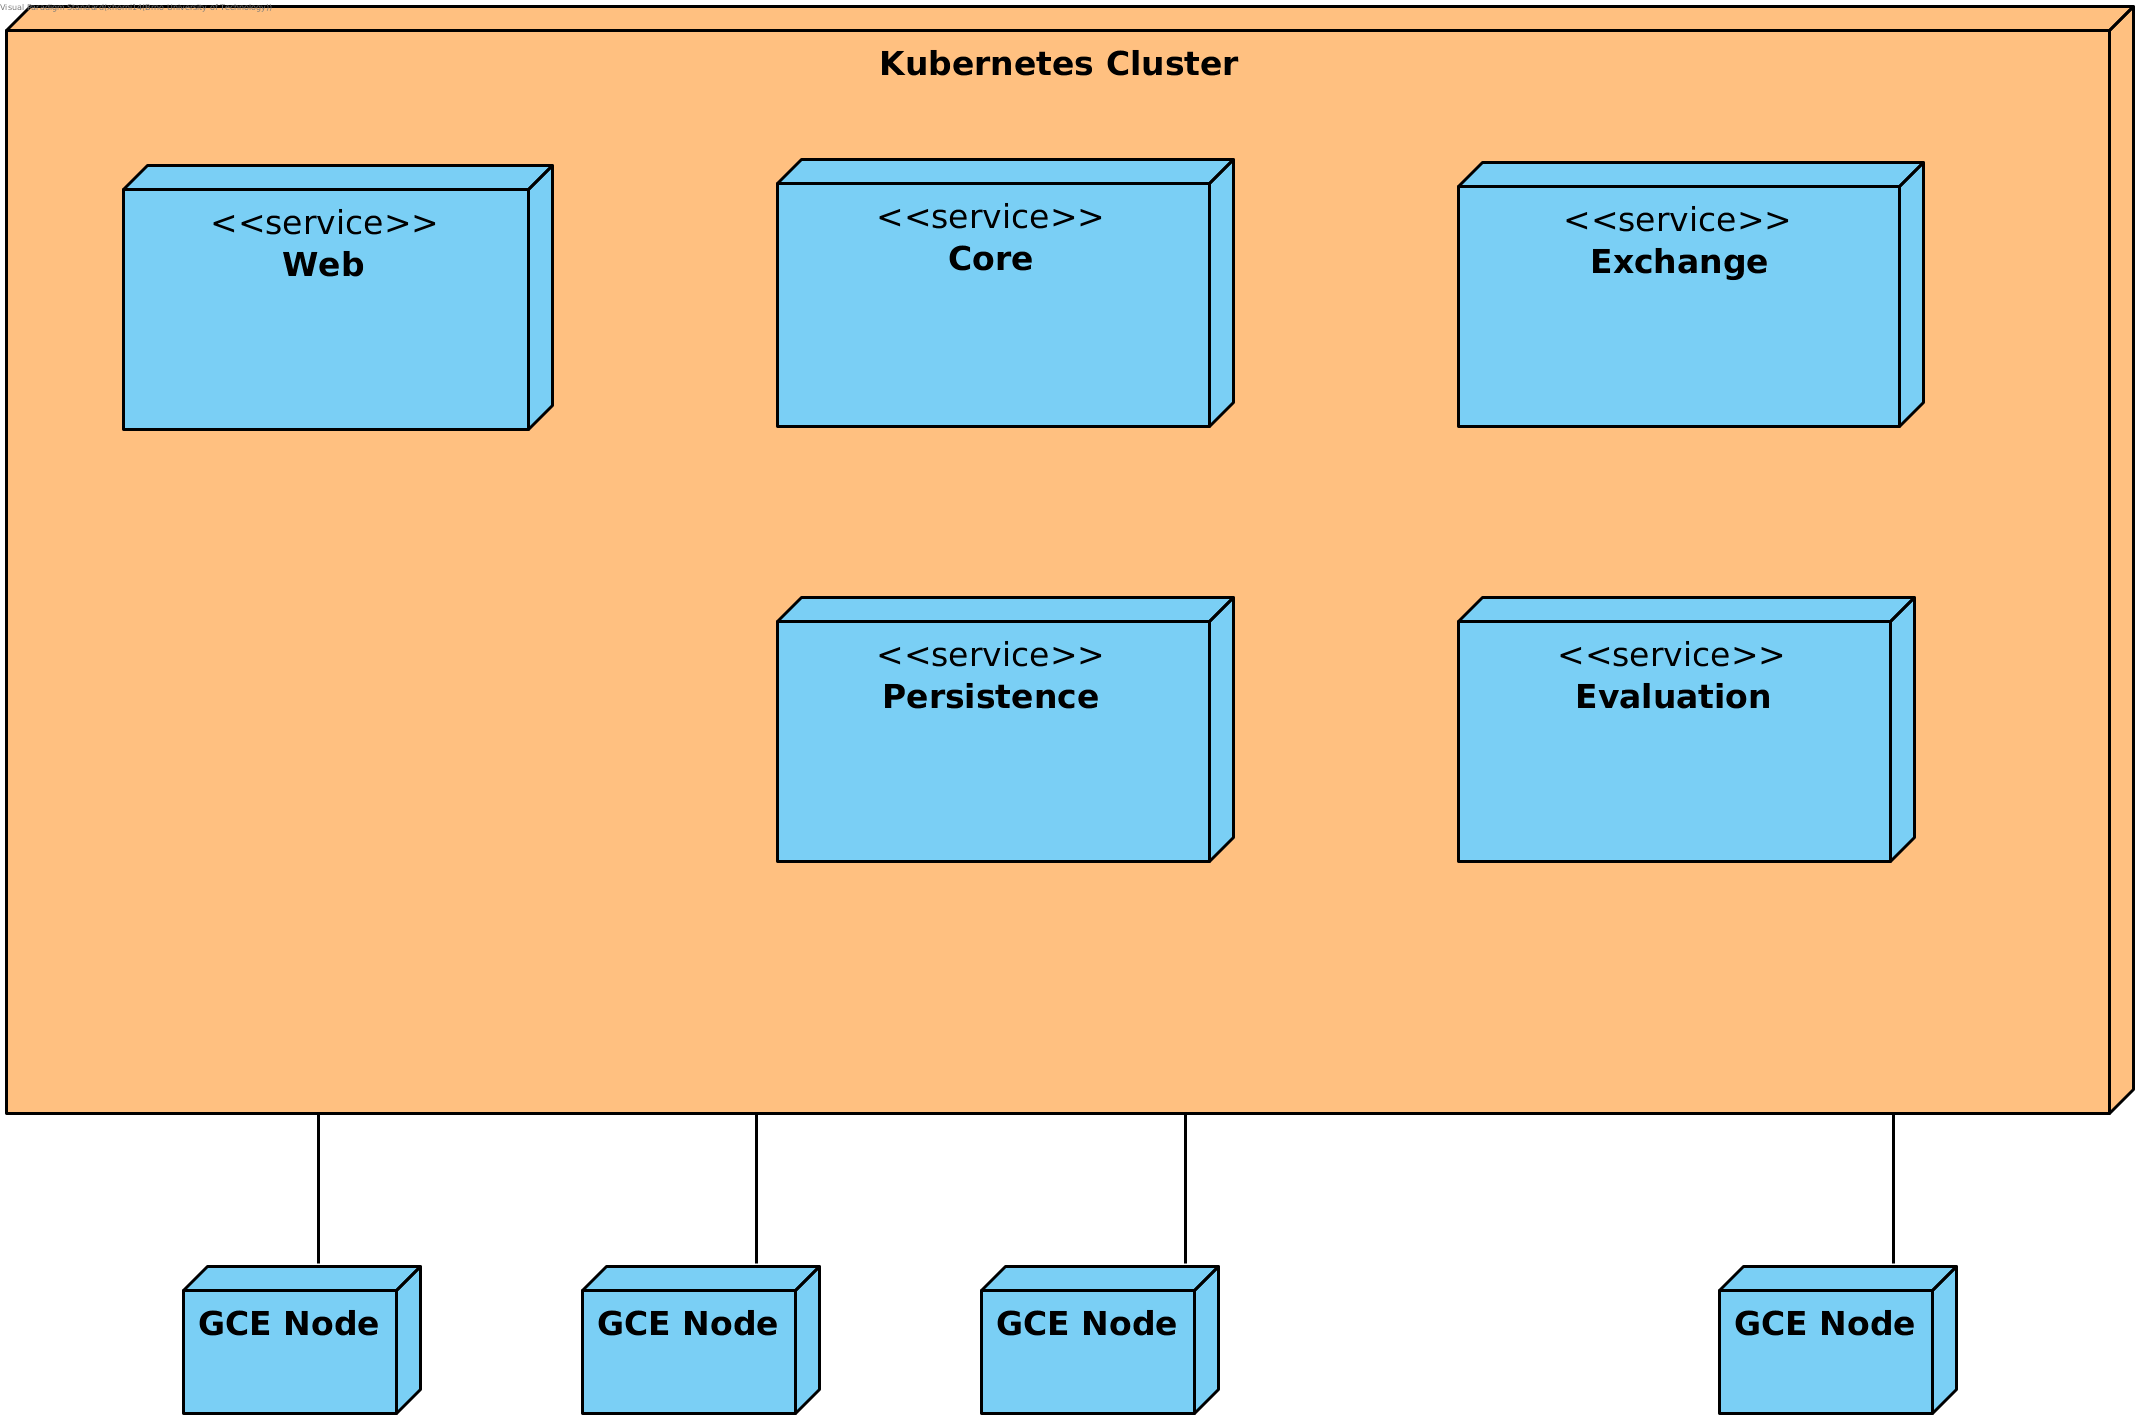
\includegraphics[width=\textwidth]{obrazky-figures/Deployment Diagram1.png}
    \caption{Basic architecture}
    \label{img:arch}
\end{figure}


\section{Component design}
By using Kubernetes we virtualized the computing environment. The environment as perceived by individual components
will just be a set of connected Docker containers with access to DNS server, that contains information about other components.
Kubernetes also provides virtualized network environment, making it appear as if all containers were on a same network.

This fact greatly simplifies architectural challenges. The only architectural challenge remaining, is the definition
of how will the application components be connected and communicate. While the actual communication protocol is
defined later in this chapter, here we are interested in more conceptual approach.

Application is divided into several components:
\begin{itemize}
    \item Web component - Provides a web interface for users' inetraction with the system, and interacts with the database
    \item Core component - Accepts input from users, incoming data from exchanges, decides when to evaluate strategies, and when to create orders on exchanges
    \item Evaluation component - Evaluates strategies based on requests from Core service
    \item Persistence component - Stores tick data and user data upon provided by core service, and provides this data to all services if necessary
    \item Exchange components - Each of these components serves as an adapter, that connects to external exchange API, and
    maps its specific API onto internal communication channels.
\end{itemize}

\begin{figure}[H]
    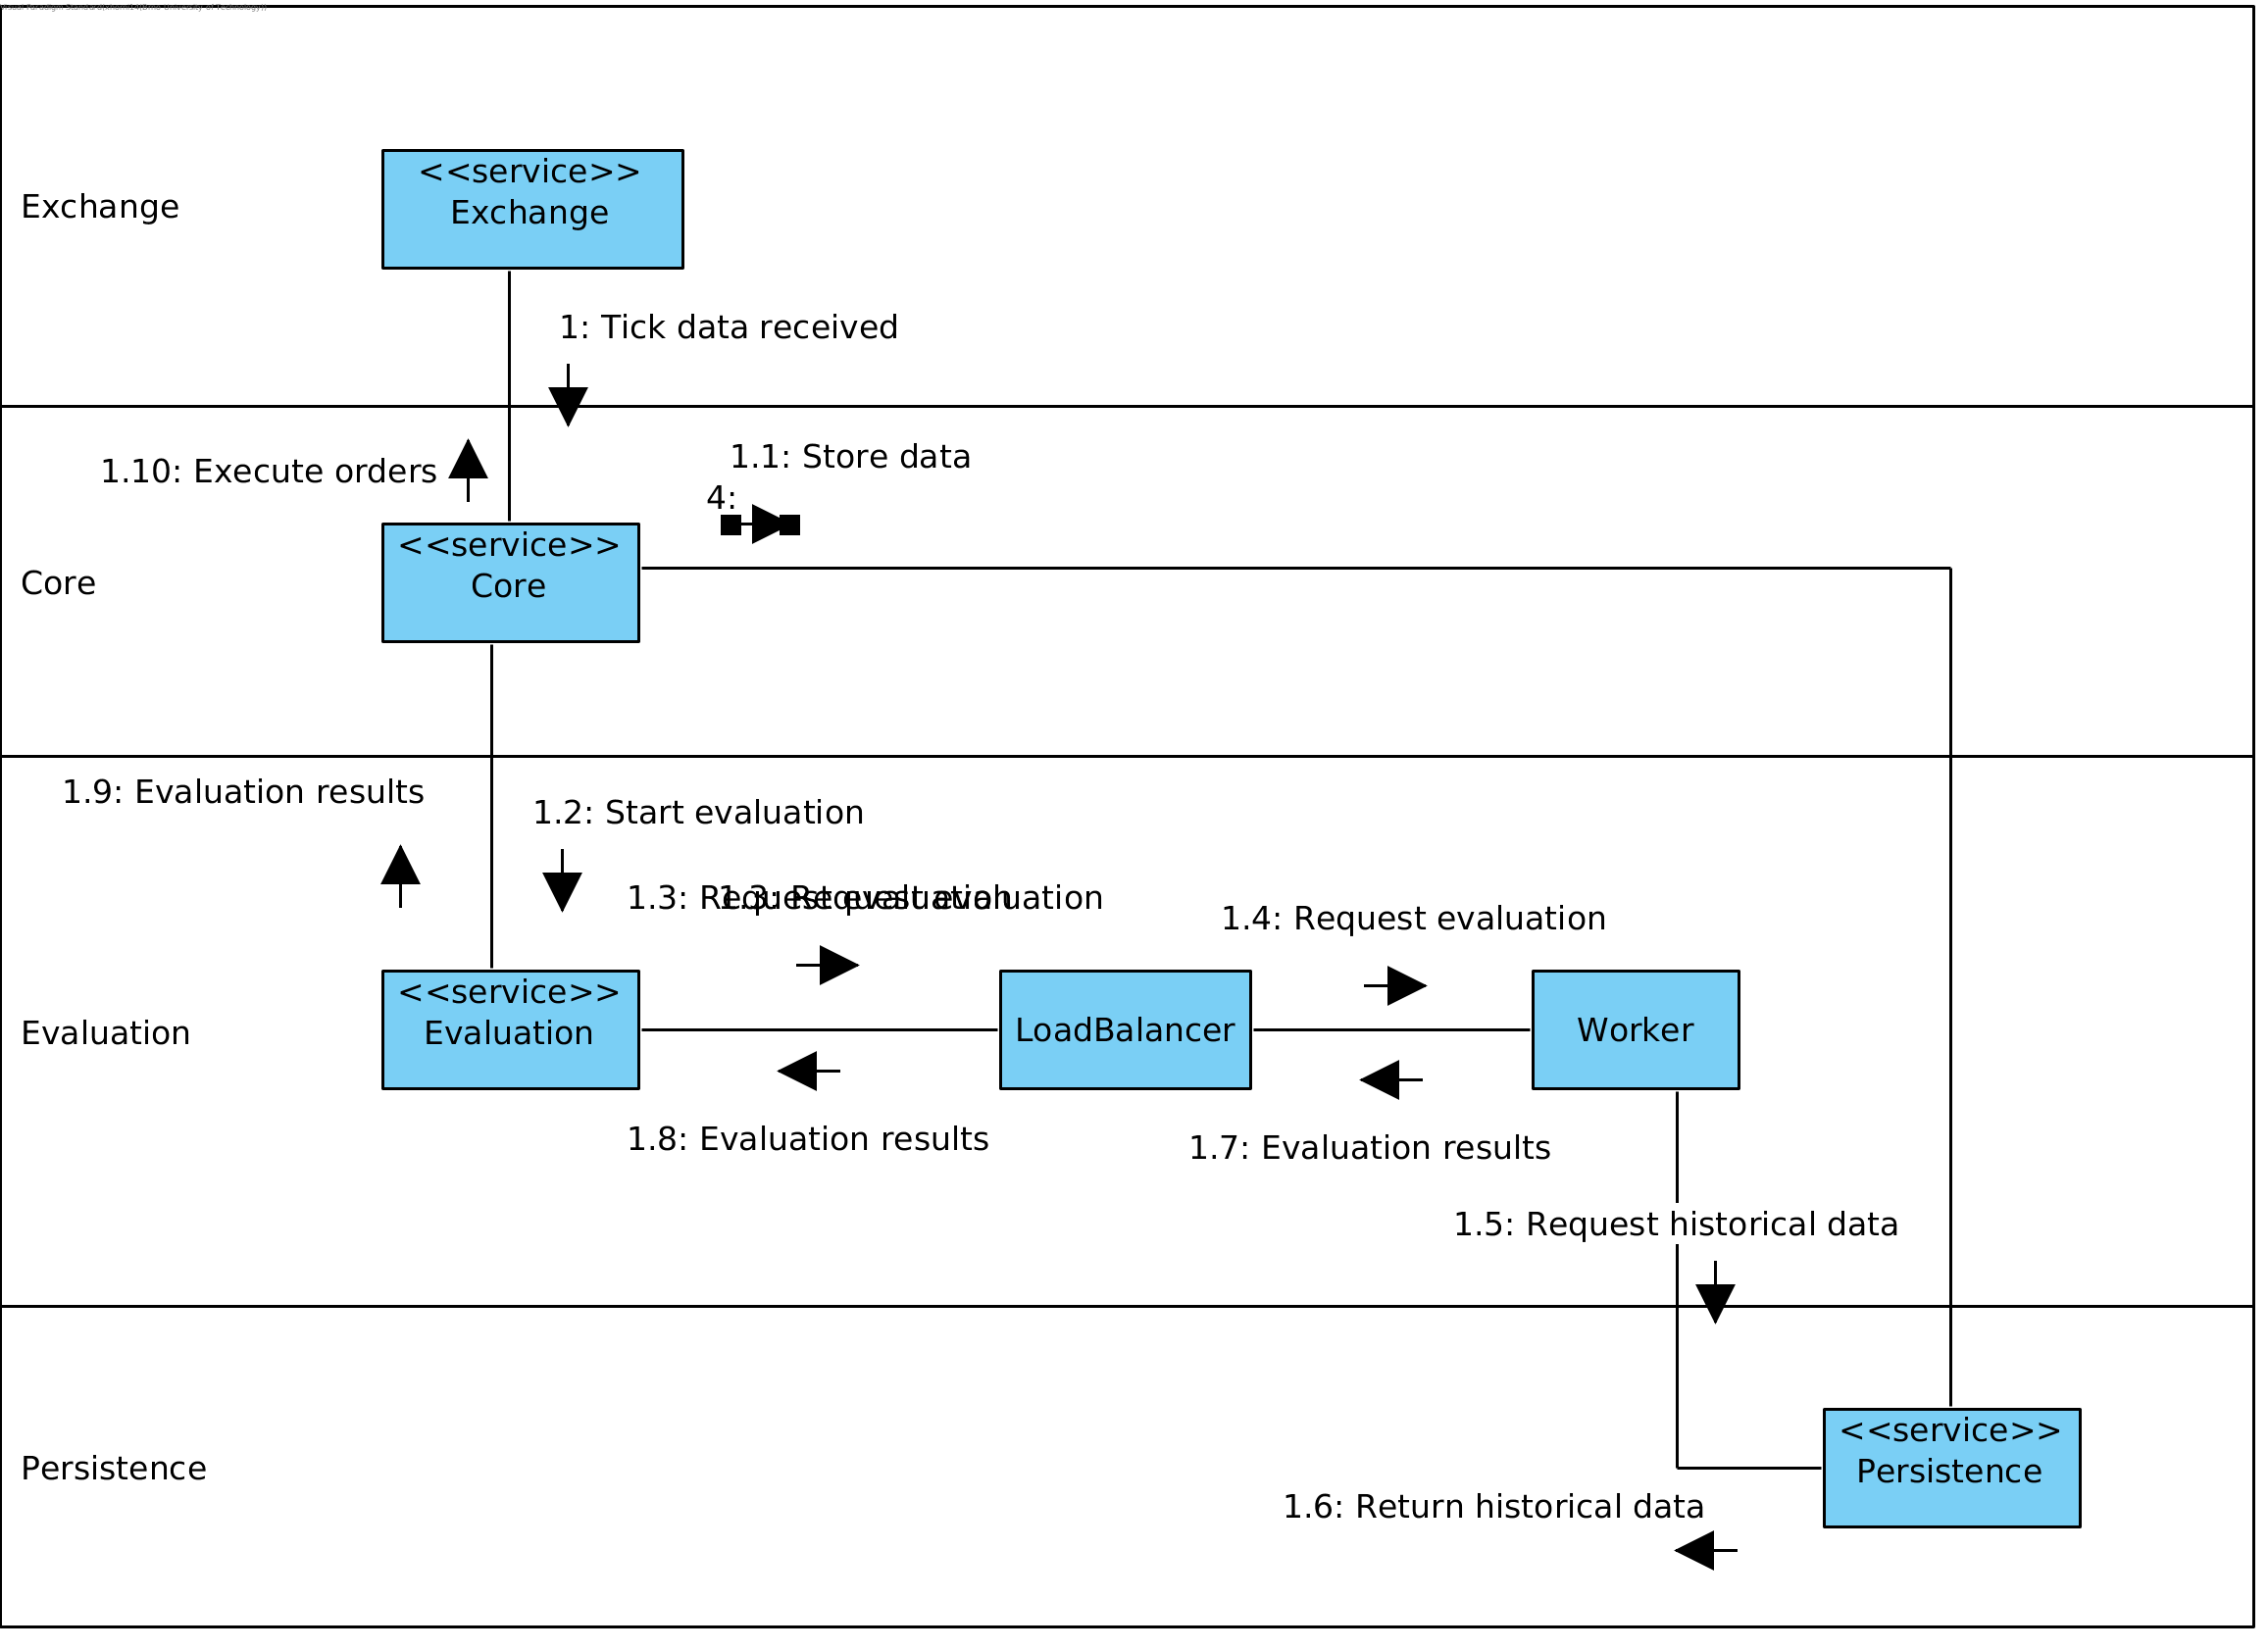
\includegraphics[width=\textwidth]{obrazky-figures/Service communication diagram.png}
    \caption{Service communication diagram}
    \label{img:service_comm}
\end{figure}

\autoref{img:service_comm} shows a communication diagram that describes communication between individual services, that
will occur in response to receiving new financial data from an exchange. The system will store this information
into persistent storage for later use, and if the information is up to date, it will initiate strategy evaluation
for strategies applied to currency of incoming data.

\subsection{Individual component architecture}
Each of these services will be comprised of one or more kubernetes \kubecomp{service}-\kubecomp{deployment} pairs. The
\kubecomp{service} part will ensure availability of information about individual pods on kubernetes' internal DNS server.
The \kubecomp{deployment} part will ensure the availability of actual pods.

Each service will be comprised of one ore more \kubecomp{pods} that will be managed by \kubecomp{deployment}. Each \kubecomp{pod}
will contain base communication actor from \verb|actix-comm| library, and several other actors to support communication with other services. In addition to
these supporting actors, it will also contain varying number of actors, that will collectively implement
the desired functionality of a particular component.

\section{Communication \& actix-comm}
\label{section:actix_comm}
As described earlier the Actix library does not provide tools for communication between actors on different machines. One of the
goals of this thesis was to design \& implement a library that would facilitate this functionality. The resulting library
should be usable by other projects.

\subsection{Underlying protocol}
We chose to use ZeroMQ\cite{hintjens2011} as an underlying protocol instead of TCP/UDP because of several factors. The ZeroMQ can be used over
many different transport types, including TCP, UDP, Unix pipes, PGM or shared memory. Another benefit is the added flexibility; While
TCP requires estabilishing connection in a particular order (Bind then Connect), while ZeroMQ does not have similar constraints.

It also provides wide array of socket types to implement different communication paradigms. We primarily use 2 of them.

The Router-Dealer socket pair is well suited for asynchronous request-reply communication pattern, and will be most commonly used as
such.

\todo{Reword}
The Pub-Sub socket pair will be used for pub-sub communication pattern. This communication pattern will be used for receiving
large amounts of financial data from exchanges, and maybe for some additional system functions, like logging.

\subsection{Library interface}
Because the library is intended to be used exclusively with the Actix framework, the only provided interface will be in form
of a several actors. These actors will respond to a set of messages that are also exported by the library. These messages
are of 2 types, control, and data messages. Control messages will affect the state of one or more communication actors
in one process, and data messages are requests to send data to different processes/machines.

The implementation of additional functionality by creating a set of actors \& messages is is very common within the actix ecosystem.
The actix-web library, which is used to implement the web application, is also built with similar approach

\todo{Rewrite - Not accurate anymore}
\subsection{Communication protocol}
The library imnple
Each component will utilize several ZeroMQ sockets. The primary socket will be of Dealer type, and will serve as an endpoint
for accepting connections from other components. In addition to one Dealer socket, each component will alse create a router
socket for each connection to another component. The requests will be sent over this router socket.

\begin{figure}[H]
    \includegraphics[width=\textwidth]{obrazky-figures/actix-net communication.png}
    \caption{actix-comm communication}
    \label{img:actix_comm}
\end{figure}

In \autoref{img:actix_comm} you can see simple sequence diagram showing types of most common interactions with the library. The \actor{Communicator}
actor serves as a entry point into the library. By creating and sending \msg{Connect} message to this actor, the \actor{Node} actor is created,
and the address of created node is retruned into user code. User can use the \actor{Node} actor for sending messages to
remote nodes. User can register global handlers for specific message type
using the \msg{RegisterRecipient} message, and specific actors using the \msg{RegisterActor} message. The response to \msg{RegisterActor}
message is global actor address, which can be sent to other nodes, and used to send messages to specific actor on local node.


\subsection{Actix-arch}
Is a library that was built on top of \verb|actix-comm| simplify development of individual components. It contains implementations
from commpon communication patterns, and components to support the development of communicating applications.

\subsubsection{Service abstraction}
Since most common communication pattern is Request-Response, this component was created to support this type of communication.
It consists of 3 parts. The \trait{ServiceInfo} trait, that is used for declaring crucial information about the service, like
hostname, on which the service is available, and types of request and response.

%@formatter:off
\begin{code}[language=rust,label={svcinfo_trait},caption={ServiceInfo trait definition}]
pub trait ServiceInfo: 'static + Debug {
    type RequestType: Remotable + Debug;
    type ResponseType: Remotable + Debug;
    const ENDPOINT: &'static str;
}
\end{code}
%@formatter:on

Two other components are the \type{ServiceHandler}and \type{ServiceConnection} actors, which are generic over type paramenter
S, that must implement \trait{ServiceInfo} trait, that describes the service that component handles or connects to.
The \type{ServiceHandler} struct has a register method, which can be used to register a handler of service messages.
Both of these structs internally use ZeroMQ actors defined in \verb|actix-comm| library, namely the Request and Reply actors.

\subsubsection{Publish - subscribe abstraction}
Is an apstraction for implementing Publish-Subscribe data flows.
Is analogous to Service abstraction, utilizing 3 parts. The \trait{EndpointInfo} trait defines the hostname, on which
the binding endpoint can be found, its associated type \type{FanType} can be either \type{FanOut} or \type{FanIn},
and defines, which part of the communication channels binds to an address, and which connects to it.
With \type{FanIn}, the subscriber binds to a port, and multiple publishers connect to it (used for receving tick
data from multiple exchange adapters), and with \type{FanOut}, the publisher binds to a socket, and subsribers connect
to it.

%@formatter:off
\begin{code}[language=rust,label={endpointinfo_trait},caption={EndpointInfo trait definition}]
pub trait EndpointInfo {
    type MsgType: RemoteMessage<Result=()> + Remotable;
    type FanType: FanType = FanOut;
    const ENDPOINT: &'static str;
}
\end{code}
%@formatter:on

The \type{Publisher} and \type{Subscriber} actors are generic over type paramenter E, that must implement the \trait{EndpointInfo}
trait, and contain methods for publishing and subscriving to updates respectively.

\subsubsection{Service load balancing}
Other component necessary for our designed system was a way to perform load balancing for Service handlers.
This will be mainly used in the strategy evaluation component, since this component will probably result in most
of the computing load.

This component is implemented as 2 actors: the \actor{LoadBalancer} and \actor{WorkerProxy}, which botha have one type
parameter S that must implement ServiceInfo. Then, the LoadBalancer binds 2 ServiceHandlers to single port.
The first one is used for receiving service requests from client, and the second one is used for receiving message for workers.

The workerProxy internally contains a \type{ServiceConnection}, that connects to \actor{LoadBalancer}, and periodically subscribes
for work. If \actor{LoadBalancer} does not have any work available, it sends an empty response to \actor{WorkerProxy},
or, if available, it sends a work unit to this worker. The \actor{WorkerProxy} then sends received work to internal
worker implementation, and after finishing, sends result to \actor{LoadBalancer} as a separate request, that is also used
for requesting more work units.

The \actor{LoadBalancer} therefore serves as a load balancing broker, which performs rendezvous between available workers
and work units, communication using 2 service handlers.

\section{Data storage}
Another crucial aspect of designed system is the storage of both the financial data and general system data.
These 2 types of data have different storage requirements.

\subsection{Financial data}
\todo{Move this earlier ?}
Financial data received from exchanges is in the form of several prices and volume that is aggregated over a time interval.
These prices are:
\begin{itemize}
\item{Open - } Price, that was used in first transaction in this time interval
\item{High - } Highest price that was used in transaction in this time interval
\item{Low - }  Lowest price that was used in transaction in this interval
\item{Close -} Price, that was used in last transaction in this time interval
\end{itemize}
In adition the these price, each interval is associated with its starting timestamp, and cumulative volume
of executed trades. We will refer to this type of data as OHLC data, based on the OHLC chart which is used for displaying
these datasets (\todo{Footnote https://www.investopedia.com/terms/o/ohlcchart.asp}).

There are several requirements put on storage solution that will be used for storing the OHLC data, mainly stemming from
amount of this data, and operations that must be performed on it.

The chosen storage solution will have to support large ingest rates. For most basic implementation, supporting bitfinex exchange,
we will have to store OHLC data for almost 100 assets, most of which are updated every 10 seconds. This would mean
the insert rate of 10 rows per second.

Another aspect is periodic retrieval of latest data for evaluation of strategies. This retrieval is not a simple load from database,
the stored data will have to be cleaned up,
\todo{Insert missing mpoints}

\subsection{Application data}
For storing application data, we have to store data that conforms to relational model.
\todo{ERD HERE}
This ERD diagram shows basic data model of the system. This data model utilizes several foreign keys, and will require
a relational database for storage.

\subsection{Evaluated storage solutions}
In order to store application data, we just have to use a relational database. These databases are most common types of databases used,
and have extensive tooling built to support them. For the purposes of this application the \textbf{PostgreSQL} databases was chosen.
This is an open source database which supports most of the modern SQL, and probably the only competitor to Oracles offering
in terms of functionality. One of the most exciting features of this database is support of extensions, that transform
this simple relational database into general purpose storage solution. Some of the database extensions are
\begin{itemize}
    \item Citus - Adds support for clustered deployments, in which several instances of PostgreSQL databases store
        data - improving redundancy and performance
    \item TimescaleDB - Improves upon built-in table partitioning, and adds custom storage engine optimized
        for time-series datasets.
    \item Cstore - Adds columnar store, which can be used for storing data in ORC format.
\end{itemize}
Thanks to these features, the \textbf{PostgreSQL} was chosen as a database for storing application data.

However, the storage solution for storing OHLC data has different requirements. The chosen solution will have
to support large insert rates mentioned earlier, fast retrieval of newly inserted subset of data, and preservation
of these properties over time, when amount of stored data grows past the amount that could be stored in memory.

These requirements are common among the applications that deal with a steady stream of time-dependent data, also called
time-series data.

There are several approaches to storing time-series data. We could store it as a normal postgresql table.
This would ensure avaiability of analytical functions for working with data in the database engine, removing the
need to implement it in application. But the drawback of this approach is scalability. While \textbf{PostgreSQL} is
among the most peroformant database today, its performance quicky degrades with large tables\todo{Cite timescaledb research on
ingest rates}. Most common solution to this problem is table partitioning, that creates sub-tables for our time-series
data table, and divides data into these subtables based on the temporal dimension. However, this requires additional
tooling and management.

Another approach is to use a distributed database with multiple nodes. Then, the data would be partitioned across multiple nodes,
with some degree of redundancy. Therefore, inserts and reads both can be easily parallelized, and we would gain redundancy,
preserving data in case of node failure. Drawback of this approach is the overhead, that will use of multiple nodes incur.
\textbf{ScyllaDB} was evaluated as an alternative, that utilizes the distriubuted approach.

But, after considering these multiple approaches, we have decided to use \textbf{PostgreSQL} with the \textbf{TimescaleDB}
extension for storing OHLC data. The \textbf{TimescaleDB} extension targets time-series data storage, making it ideal for our needs.
It creates a \textit{hypertable} concept, that is an abstraction over standard table, perfrorming automatic partitioning over
temporal dimension, and optionally over several hash dimensions. It also provides to analytical functions for working with time
series data (eg. \verb|time_bucket| that allows working with data over different timescales). Thanks to the
customized storage engine and automatic partitioning, this extension solves the main problem of reduced performance
for large databases.

However, if this approach fails, there is experimental \textbf{ScyllaDB} storage layer for storing OHLC data,
that seems to provide same performance as current \textbf{PostgreSQL} storage layer.

\todo {ERD}
\todo{Postgresql with timescaledb}
\todo{Hypertable - sharding}
\todo{Currently more htan enough, we'll see about future}

\todo{Experimental Scylladb backend}
\todo{Not in production, postgresql more than enough}

\subsection{Web}

\todo{Classing Client-Server SPA Design}
\todo{Usage of actix-web for Rest API}
\todo{React for frontend with material-ui}
\todo{Ace editor for editing code}
\todo{Future enhancement - websocket with live notifications}

\subsection{Exchange adapters}
\todo{Connecting to websocket}
\todo{Mapping to core using Fan-In topology}

\section{Strategies}
In \autoref{chapter:current_state} we have described several implementations of automatic trading systems. Each one of them
utilized some kind of programming language to define a trading strategy. In this regard, our system is very similar to others.

The system will have to support execution of user-written code. This fact poses a security concern. Because the user
written code can perform arbitrary actions permitted by given programming language, we must carefully choose the programming
language that will be used. Because implemented strategy will be operating with large amount of financial data, another
concern is performance. And finally, since the intended users of this application are not programmers, the chosen language
should be easy to use for beginners.

\subsection{Language choice}
These requirements severely limit possible choices. We can't accept user-compiled code, because of security concerns.
Compiled languages like C/C++ are not acceptable because of large amount of infrastructure needed to support
on-demand compilation of user written strategies.

Managed languages like Java or C\# are a better choice, but they still require large runtimes with long start up times, therefore
are not well suited for running short-lived scripts.

Scripting languages like Lua, Python or JavaScript seem like the best choice for this goal, with the drawback of
reduced performance.

\subsection{Lua}
Ultimately, the Lua language was chosen as a primary language for implementing user defined strategies. There were several
key properties, which caused this decision.

\begin{itemize}
\item Embeddability - Lua runtime is smaller than 256Kb, has virtually no start up time and can be embedded in application.
as a simple library. In comparison, neither Python nor JavaScript runtimes can be embedded in the application, and both
require large standard libraries
\item Extendability - Basic lua standard library can be easily extended with code written in host language.
\item Expressive power - While extremely simple, lua provides tools to model virtually any programming paradigm with ease
\item Speed - While lua is a scripting language, that can't possibly compete with compiled language in this space,
it is one of the fastest scripting languages available.
\end{itemize}

\subsection{Safety}
By using an intepreted language for implementation of user strategies, we have successfully eliminated a whole
class of risks. By using a safe language, the probability of user code crashing the executing process is virtually
none. However, there still are several safety issues, that have to be resolved, even with using an interpreted language.
\todo{Safety - Creating safe environment withouyt file access, Limit execution time}

\section{Evaluation}
Since users can crate multiple strategies, and then apply these trategies to multiple different assets on different exchanges,
the amount of work associated with a single user can vary extremely. In addition to that, the number of users of our system can vary.
This variability of computational load on the system was primary reason for designing the system as a distributed application.

The service that is most affected by this variability is the strategy evaluation service. This service needs to
dynamically change the amount of used resources.

This will require specific architecture. The service will be divided into 2 parts. The control and the worker layers.
The control layer will be a single Kubernetes pod, that will serve as an endpoint to rest of the system. It will receive
strategy evaluation requests from Core service, and will pass them to individual workers int the worker layer.
Each worker will be a single pod with multiple worker actors, each of which will register itself with control layer.

The control layer will also perform load balancing, ensuring that no single worker is over- or underutilized.

\todo{Eval balancer implemented as a load balancing broker}

\todo{TA library used to provide basic indicatiors (optimized) - Otherwise an iterator over raw values is available,
user can manuall implement his logic}

Then, the kubernetes horizontal pod autoscaler\footnote{\url{https://kubernetes.io/docs/tasks/run-application/horizontal-pod-autoscale/}} will be used to dynamically adjust number of pods. In addition to that,
the Google Kubernetes Engine also supports automatic node provisioning, meaning we can automate every part of scaling the system
compute capabilities.

\chapter{Implementation}
\todo{Implemented using rust}
\todo{Rust version - Features used}
\todo{Global architecture - Packages - Common, deps and app/web}

\todo{Persistence - ERD}
\todo{Needs to be first do better understand other components}

\section{Bitfinex adapter}
\todo{Implemented in deps library - apis }
\todo{Other exchanges similar}


\section{Core component}
\todo{Ingest - Cleanup }
\todo{Rescaler - Generation of virtual ohlc values}
\todo{Decision - Loads assignemnts from database, }

\section{Eval}
\todo{Balancing broker - Implementation in actix-arch - detail }
\todo{Worker - Connects to broker, internally a ServiceHandler}
\todo{Upon request - Loads OHLC + Strategy data from db}
\todo{Ohlc - Complex query - performs backfilling - rescaling}
\todo{Instantiates Lua VM, executes}
\todo{TA library}

\section{Trader component}
\todo{Receives requests for trades }
\todo{Forwards to individual exchanges}
\todo{Generic positionService provided by exhcnages}
\todo{First the balanceServicea to get wallet balances}
\todo{THen TradeService to execute trades and ensure target position}

\todo{Everything logged into}

\section{Persistence component}
\todo{Implemented in the DB library}
\todo{Uses diesel for query generation}
\todo{Synchronous - uses R2d2 for connection pooling and SyncActors for concurrent access to DB}

\todo{Experimental storage of OHLC data in ScyllaDB}


\section{Web component}
\todo{Backend - Actix web with diesel entities }
\todo{Simple Crud - Usage of Database actor - the invoke method}

\subsection{Frontend}
\todo{React - basics}
\todo{Redux for state management}

\section{Deployment and Management}
\todo{Describe ops}
\todo{Deployment process using opnmly makefiles and kubernetes config}
\todo{Docker image creation}
\todo{Tagging by hash for debug, by git for release}

\todo{Monitoring using kubernetes dashboard}


\chapter{Testing and evaluation}
\todo{Application logging}
\todo{Debugging using telepresence and local components}


\section{Evaluation}
\todo{A few strategies - latency}
\todo{Grow strategies - latency}
\todo{Add more nodes - latency}
\todo{should be at most logarithmic - DB will be problem}


\chapter{Conclusion \& Future work}
The title of this thesis is a Design and development of distributed system that would perform a specific function.
Most of the work performed so far was design of the system, and implementation of supporting technologies. The
future development plan starts with finishing the \verb|actix-comm| library. Then, designing and implementing a persistence
service that would resolve bottlenecks found in current solution.

After issues with this part of the system are resolved, the next step will be implementation of the strategy evaluation service,
and implementation of order execution functionality into exchange service. These 2 changes will make the system able to perform its
primary function, that being automatic trading based on a strategy.

Next step will be the implementation
of the web application that will make the system implemented in previous step accessible to users. This involves the implementation of user management,
and inclusion of user data into the rest of the system.

After the web application implementation is complete, the performance of implemented system will be measured. The target of the measurements
will be the latency between system receiving new financial data, and system being able to execute orders resulting from
evaluation of strategies using this new data. The measurements will be performed with different amount of
load on the system, but the system configuration will not be changed. The expected result of these measurements is the
invariance of system latency based on system load.



